\documentclass[18pt]{beamer}
\usepackage{templates/beamerthemekit}
\usepackage[export]{adjustbox}
\usepackage{tikz}
\usepackage{url}


\title[State of the Art]{Towards Bringing Together Numerical Methods for Partial Differential Equation and Deep Neural Networks}
\subtitle{State of the Art, Supervisor - Markus Hoffmann}
\author{Stanislav Arnaudov}
\institute{Chair for Computer Architecture and Parallel Processing}
\selectlanguage{english}



\usepackage[style=verbose,backend=bibtex]{biblatex}
\bibliography{bib}
\bibliographystyle{plain}

\begin{document} 

\begin{frame}
 \titlepage
\end{frame}


\section{Motivation}
\begin{frame}

  \frametitle{Problem definition and motivation}

  \begin{columns}

    \begin{column}{0.5\textwidth}
      Partial differential equation (PDEs)
      \begin{itemize}
      \item used in simulations
      \item solutions have image representation
      \item hard to solve numerically
      \end{itemize}
      \vspace{0.25cm}
      \textbf{Goal}: solve PDEs based on their image representation 
      \vspace{-0.5cm}
    \end{column}

    \begin{column}{0.5\textwidth}
      \begin{center}
        \begin{figure}[htb]
          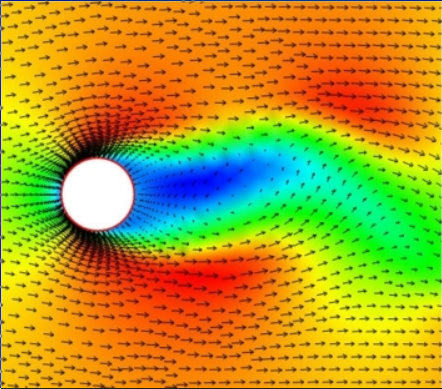
\includegraphics[scale=0.35]{images/pde}
          \caption{Flow Simulation\footnotemark}
        \end{figure}
      \end{center}
    \end{column}

    \footnotetext{``Team for Advanced Flow Simulation and Modeling'', Professor Tayfun E. Tezduyar, Sunil Sathe}
  \end{columns}
  
\end{frame}

\begin{frame}
  \frametitle{Problem definition and motivation}
  Convolutional neural networks (CNNs)
  \begin{itemize}
  \item hot topic in recent years
  \item impressive results in image processing
  \end{itemize}
  \textbf{Idea}: Use CNNs for the image representation of PDEs.
  \vspace{0.8cm}
  \begin{center}
    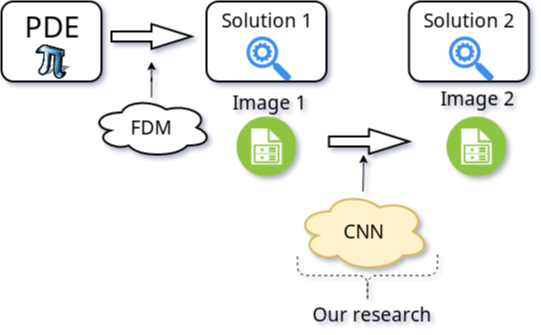
\includegraphics[scale=0.35]{images/general}
  \end{center}

\end{frame}

\begin{frame}
  \frametitle{General Goals}
  \begin{center}
    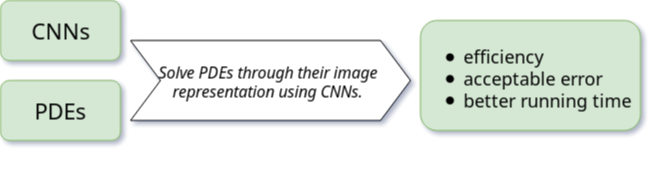
\includegraphics[scale=0.50]{images/bringing_cnn_and_pde}
  \end{center}  
\end{frame}

\begin{frame}
  \frametitle{Important Questions}

  \begin{enumerate}

  \item CNNs for image-to-image mapping?
    \vspace{0.7cm}
    \begin{center}
      
\includegraphics[scale=0.45]{images/image_to_image_cnn}
    \end{center}

    \vspace{0.5cm}
  \item CNNs for numerical simulations?
    \vspace{0.5cm}
    \begin{center}
      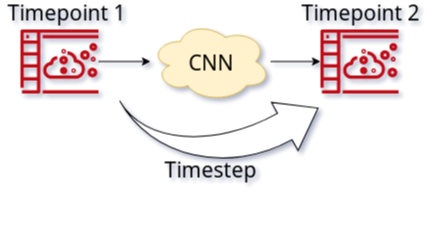
\includegraphics[scale=0.45]{images/system_to_system_cnn}
    \end{center}
    
  \end{enumerate}  
\end{frame}


\section{CNNs for image processing}
\begin{frame}
  \frametitle{CNNs for image processing}

  \begin{columns}
    \begin{column}{0.5\textwidth}
      We focus on an area where CNNs show good results:
      \begin{itemize}
      \item Image Segmentation
        \begin{itemize}
        \item pixelwise decision about a class belonging
        \item a new image is generated
        \end{itemize}
      \end{itemize}
    \end{column}
    
    \begin{column}{0.5\textwidth}
      \begin{center}
        \begin{figure}
          \centering
          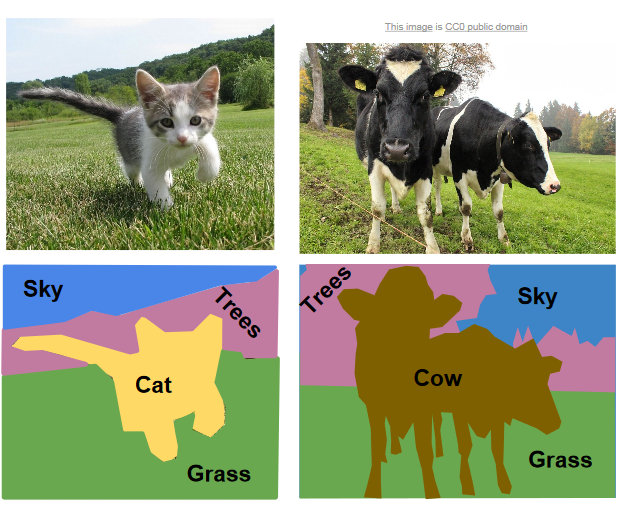
\includegraphics[scale=0.35]{images/segm}
          \caption{Image Segmentation\footnotemark}
        \end{figure}
      \end{center}
    \end{column}
  \end{columns}

  \footnotetext{``Exploring Computer Vision in Deep Learning: Object Detection and 
    Semantic Segmentation'', Long et al.,SAS Institute Inc.}

\end{frame}

\begin{frame}
  \frametitle{CNNs for image processing}
  Image segmentation
  \begin{itemize}
  \item ``Fully Convolutional Networks for Semantic Segmentation''\footcite{long2014}
    \begin{itemize}
    \item Encoder-Decoder Architecture
    \item Only convolutional layers
    \end{itemize}
  \end{itemize}
  \vspace{0.5cm}
  \begin{center}
    \begin{figure}[htb]
      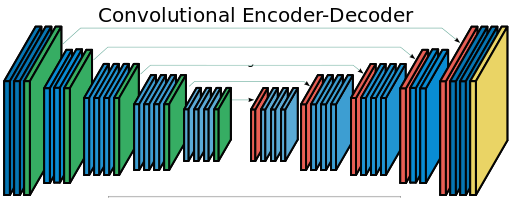
\includegraphics[scale=0.35]{images/auto_enc}
      \caption{The encoder-decoder network}
    \end{figure}
  \end{center}
\end{frame}


\begin{frame}
  \frametitle{CNNs for image processing}

  Image segmentation
  \begin{itemize}
  \item ``Semantic Segmentation using Adversarial Networks'' \footcite{luc2016}
    \begin{itemize}
    \item Generative Adversarial Networks\footcite{goodfellow2014}
    \item The Discriminator Network enforces contagiously segmented regions
    \end{itemize}
  \end{itemize}
\end{frame}

\begin{frame}
  \frametitle{CNNs for image processing}
  \begin{center}
    \begin{figure}[htb]
      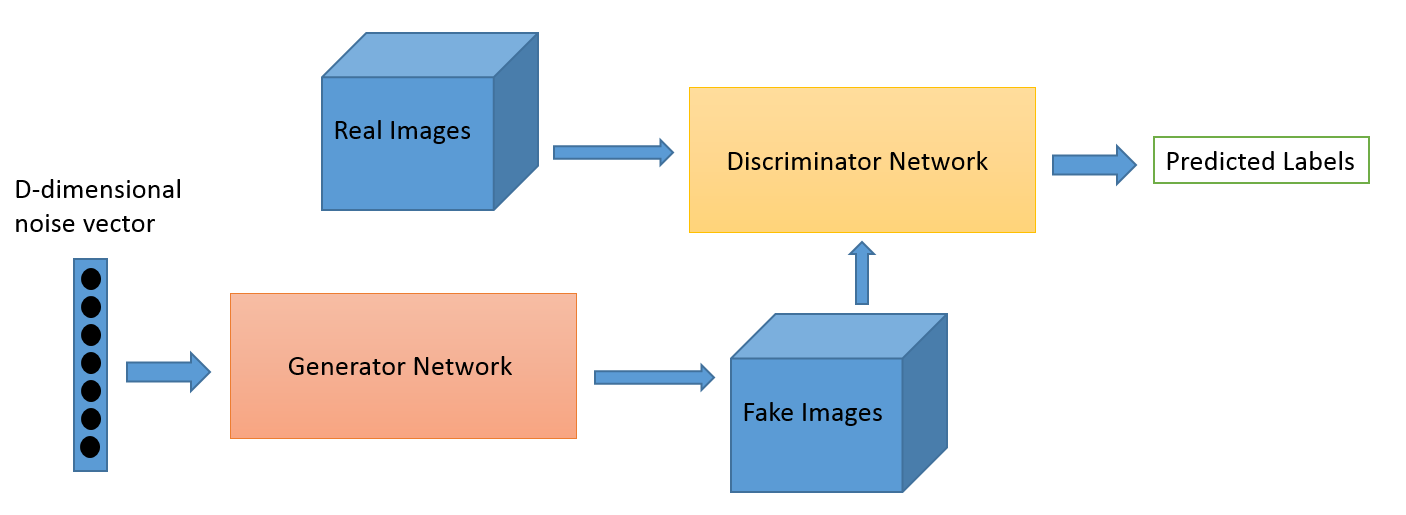
\includegraphics[width=11cm,height=5cm]{images/gan}
      \caption{Generative Adversarial Network\footnotemark}
    \end{figure}
  \end{center}
  \footnotetext{``A Beginner's Guide to Generative Adversarial Networks (GANs)'', \url{https://skymind.ai/wiki/generative-adversarial-network-gan} }
\end{frame}

\begin{frame}
  \frametitle{CNNs for image processing}
  Semantic Image Synthesis
  \begin{itemize}
  \item ``Semantic Image Synthesis with Spatially-Adaptive Normalization'' \footcite{park2019}
    \begin{itemize}
      \item Segmentation in reverse
    \end{itemize}

    \begin{center}
      \begin{figure}[htb]
        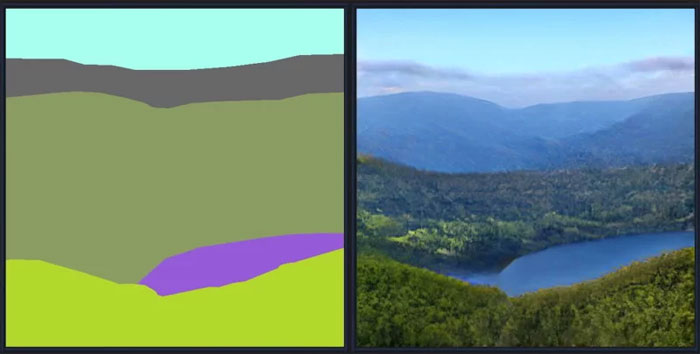
\includegraphics[width=10cm,height=3cm]{images/gaugan}
        \caption{Example of ``reversed image segmentation''}
      \end{figure}
  \end{center}
  \end{itemize}
\end{frame}



\section{CNNs for numerical applications}
\begin{frame}
  \frametitle{CNNs for numerical applications}
  Long standing interest in bringing together neural networks and formal mathematics.
  \begin{itemize}
  \item It is shown to be possible -  ``Performing basic mathematics with neurons/nets'' (2002)  \footcite{neville2002}
  \item Even for PDEs - ``Artificial Neural Networks for Solving Ordinary 
and Partial Differential Equations'' (1998) \footcite{lagaris1998}
  \end{itemize}
  
\end{frame}

\begin{frame}
  \frametitle{CNNs for numerical applications}
  Nowadays CNNs are applied to complex physical simulations.
  \begin{itemize}
  \item CNNs for calculating physical properties of objects in simulations
  \item CNNs in flow simulation
  \end{itemize}
  
\end{frame}

\begin{frame}
  \frametitle{CNNs for numerical applications}
  \begin{itemize}

  \item ``Learning Soft Tissue Behavior of Organs for Surgical Navigation with Convolutional Neural Networks''\footcite{pfeiffer2019}
    \begin{itemize}
    \item Prediction for how organs in the human body move during operation
    \item Encoder-Decoder Architecture
    \end{itemize}
    \vspace{0.25cm}
    
    \begin{center}
      \begin{figure}[htb]
        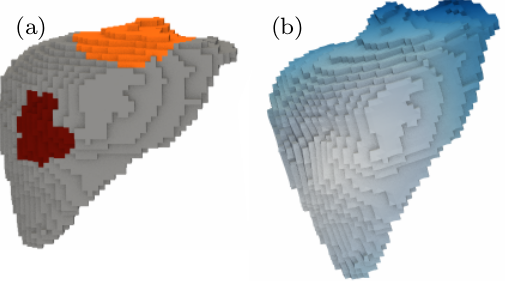
\includegraphics[scale=0.35]{images/organs_move_1}
        \caption{Given and predicted displacement of an organ}
      \end{figure}
    \end{center}
    
  \end{itemize}
  
\end{frame}
  
\begin{frame}
  \frametitle{CNNs for numerical applications}
  \begin{itemize}
  \item ``Accelerating Eulerian Fluid Simulation With Convolutional Networks''\footcite{tompson2016}
    \begin{itemize}
    \item CNN for predicting fluid-flow
    \item Calculate pressure given velocity divergence and geometry
    \end{itemize}
  \end{itemize}
  \vspace{0.1cm}
  \begin{center}
    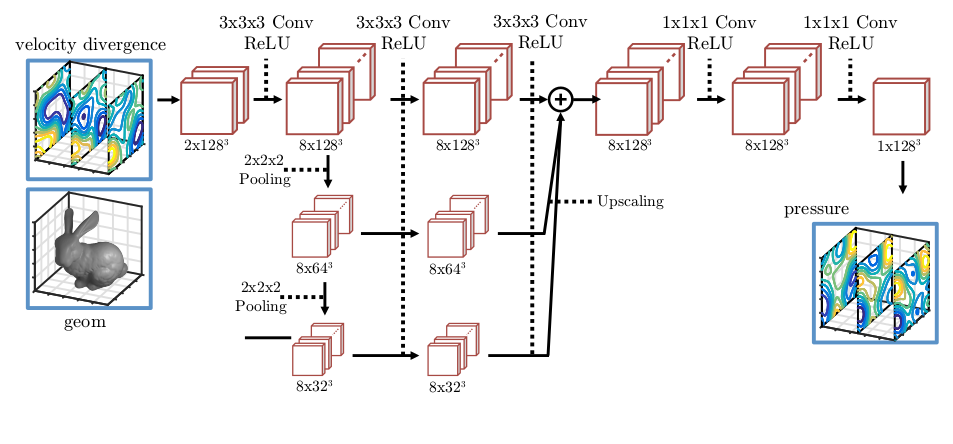
\includegraphics[width=11cm, height=4cm]{images/sim_1}
  \end{center}
  
\end{frame}
  

\section{Conclusion}
\begin{frame}
  \frametitle{Conclusion}

  To reiterate
  \begin{itemize}
  \item \textit{Problem:} Solve PDEs 
  \item \textit{Approach:} Use CNNs for image-to-image mapping
  \item \textit{Goal:} Efficiency and acceptable error
  \end{itemize}
  
  \rule{10cm}{0.4pt}
  
  The conducted research illustrates:
  \begin{itemize}
  \item A research gap
  \item Evidence suggesting the proposed method is viable
  \item Typical CNN architectures that should be considered
  \end{itemize}  
\end{frame}


\begin{frame}
  \frametitle{}
  \begin{center}
    \huge{Thank you for your attention.}    
  \end{center}
\end{frame}

\begin{frame}
  \frametitle{}
  \begin{center}
    \huge{Questions?}
  \end{center}
\end{frame}

\end{document}

%%% Local Variables:
%%% mode: latex
%%% TeX-master: t
%%% End:
